\chapter{Introduction}
\label{ch:introduction}

The constant technological developments in the automotive, sensor, and computer 
industries are empowering the development of autonomous vehicles as highly versatile
tools for civilian applications, ranging from driverless cars running in crowded 
streets and highways to the widespread use of the so-called drones in the 
motion picture industry, in agriculture, or even as a hobby.

\section{Motivation}

%-----------------------------------------------------------------------------------------
% Autonomous Helicopters
Within the scope of \glspl{acronym_uav}, autonomous rotorcraft have been 
steadily growing as a major topic of research. 
They have the potential to perform high precision tasks in challenging and
uncertain operation scenarios as new sensor technology and increasingly powerful 
computational systems are available. 
\begin{figure}
    \centering
    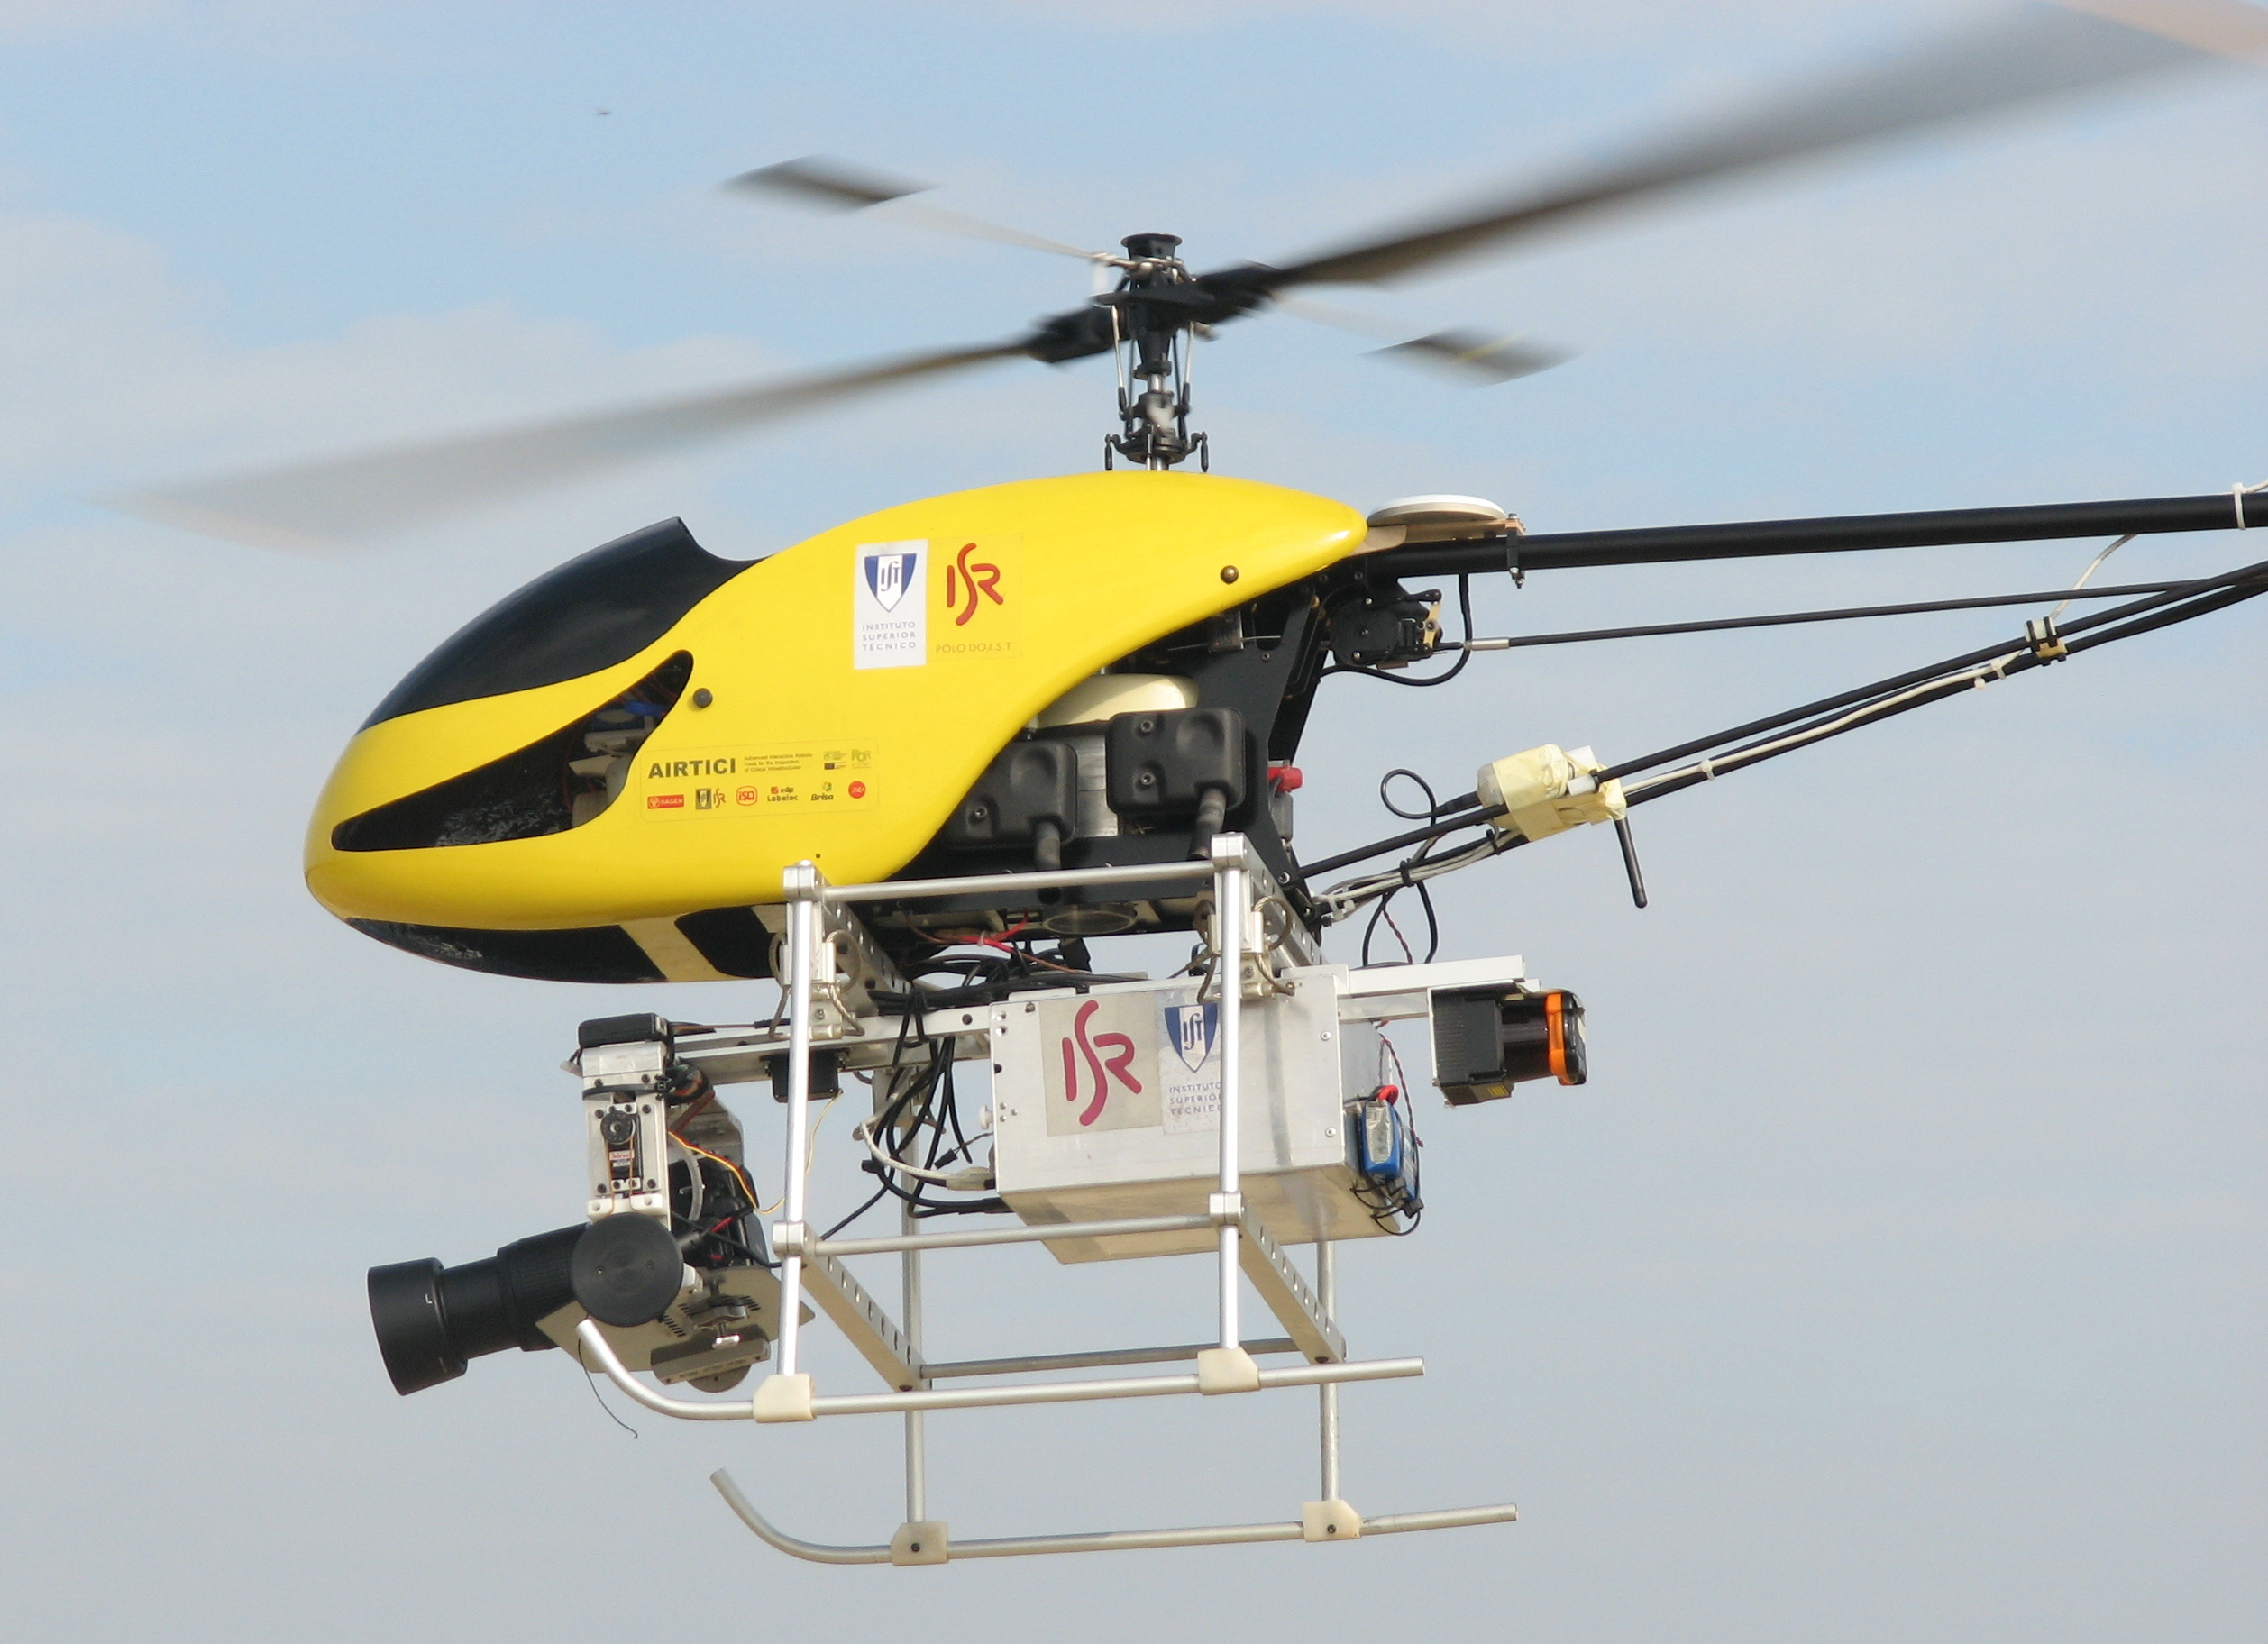
\includegraphics[width=\textwidth]{HeliFlight_bergen5.jpg}\\
    \caption{Helicopter robotic vehicle.}
    \label{fig:bergen}
\end{figure}
Missions like aerial surveillance, automatic infrastructure inspection, or
\gls{acronym_3d} surface mapping in unknown environments, demand highly adaptable
autonomous vehicles that can meet low altitude and hover flight requirements.

% Unknown environments
Reliable navigation and positioning of \glspl{acronym_uav} are fundamental for 
any autonomous mission, particularly in unknown environments where absolute 
positioning systems are absent or unreliable.
The motivation for this dissertation arises from the use of autonomous 
rotorcraft for automatic inspection of critical infrastructures and buildings, 
such as bridges, electric power lines, power plants, dams, construction areas, etc. 

The structural components of large infrastructures, such as the deck and piers of
a bridge or the walls of an industrial chimney, are affected in their strength 
and durability by age, aggressive environment, and steadily increasing operation demands, 
especially in places where design, construction, or maintenance errors have occurred 
\citep{ice:2008,chimguide:2006}. 

